\begin{frame}[label=current]
    \frametitle{Nullstellenverteilung der $\xi$-Funktion}
    \begin{lemma}
        \[\xi(s) = 0\implies 0 \leq \Re s \leq 1\]
    \end{lemma}
    \begin{proof}
        Aufgrund der Eulerproduktdarstellung gilt
        \begin{itemize}[<+->]
            \item $0 \neq \zeta(s) = \frac{\pi^{s/2}}{\Gamma(s/2)}\xi(s) \quad \forall \Re s > 1$
            \item $\implies \xi(s) \neq 0 \Leftrightarrow \xi(1-s) \neq 0\quad \forall \Re s > 1$
            \item $\implies \xi(s) \neq 0 \quad \forall \Re s < 0$
        \end{itemize}
    \end{proof}
\end{frame}
\begin{frame}[label=current]%
    \begin{figure}%
        \begin{tikzpicture}
        \node[anchor=south west,inner sep=0] (image) at (0,0) {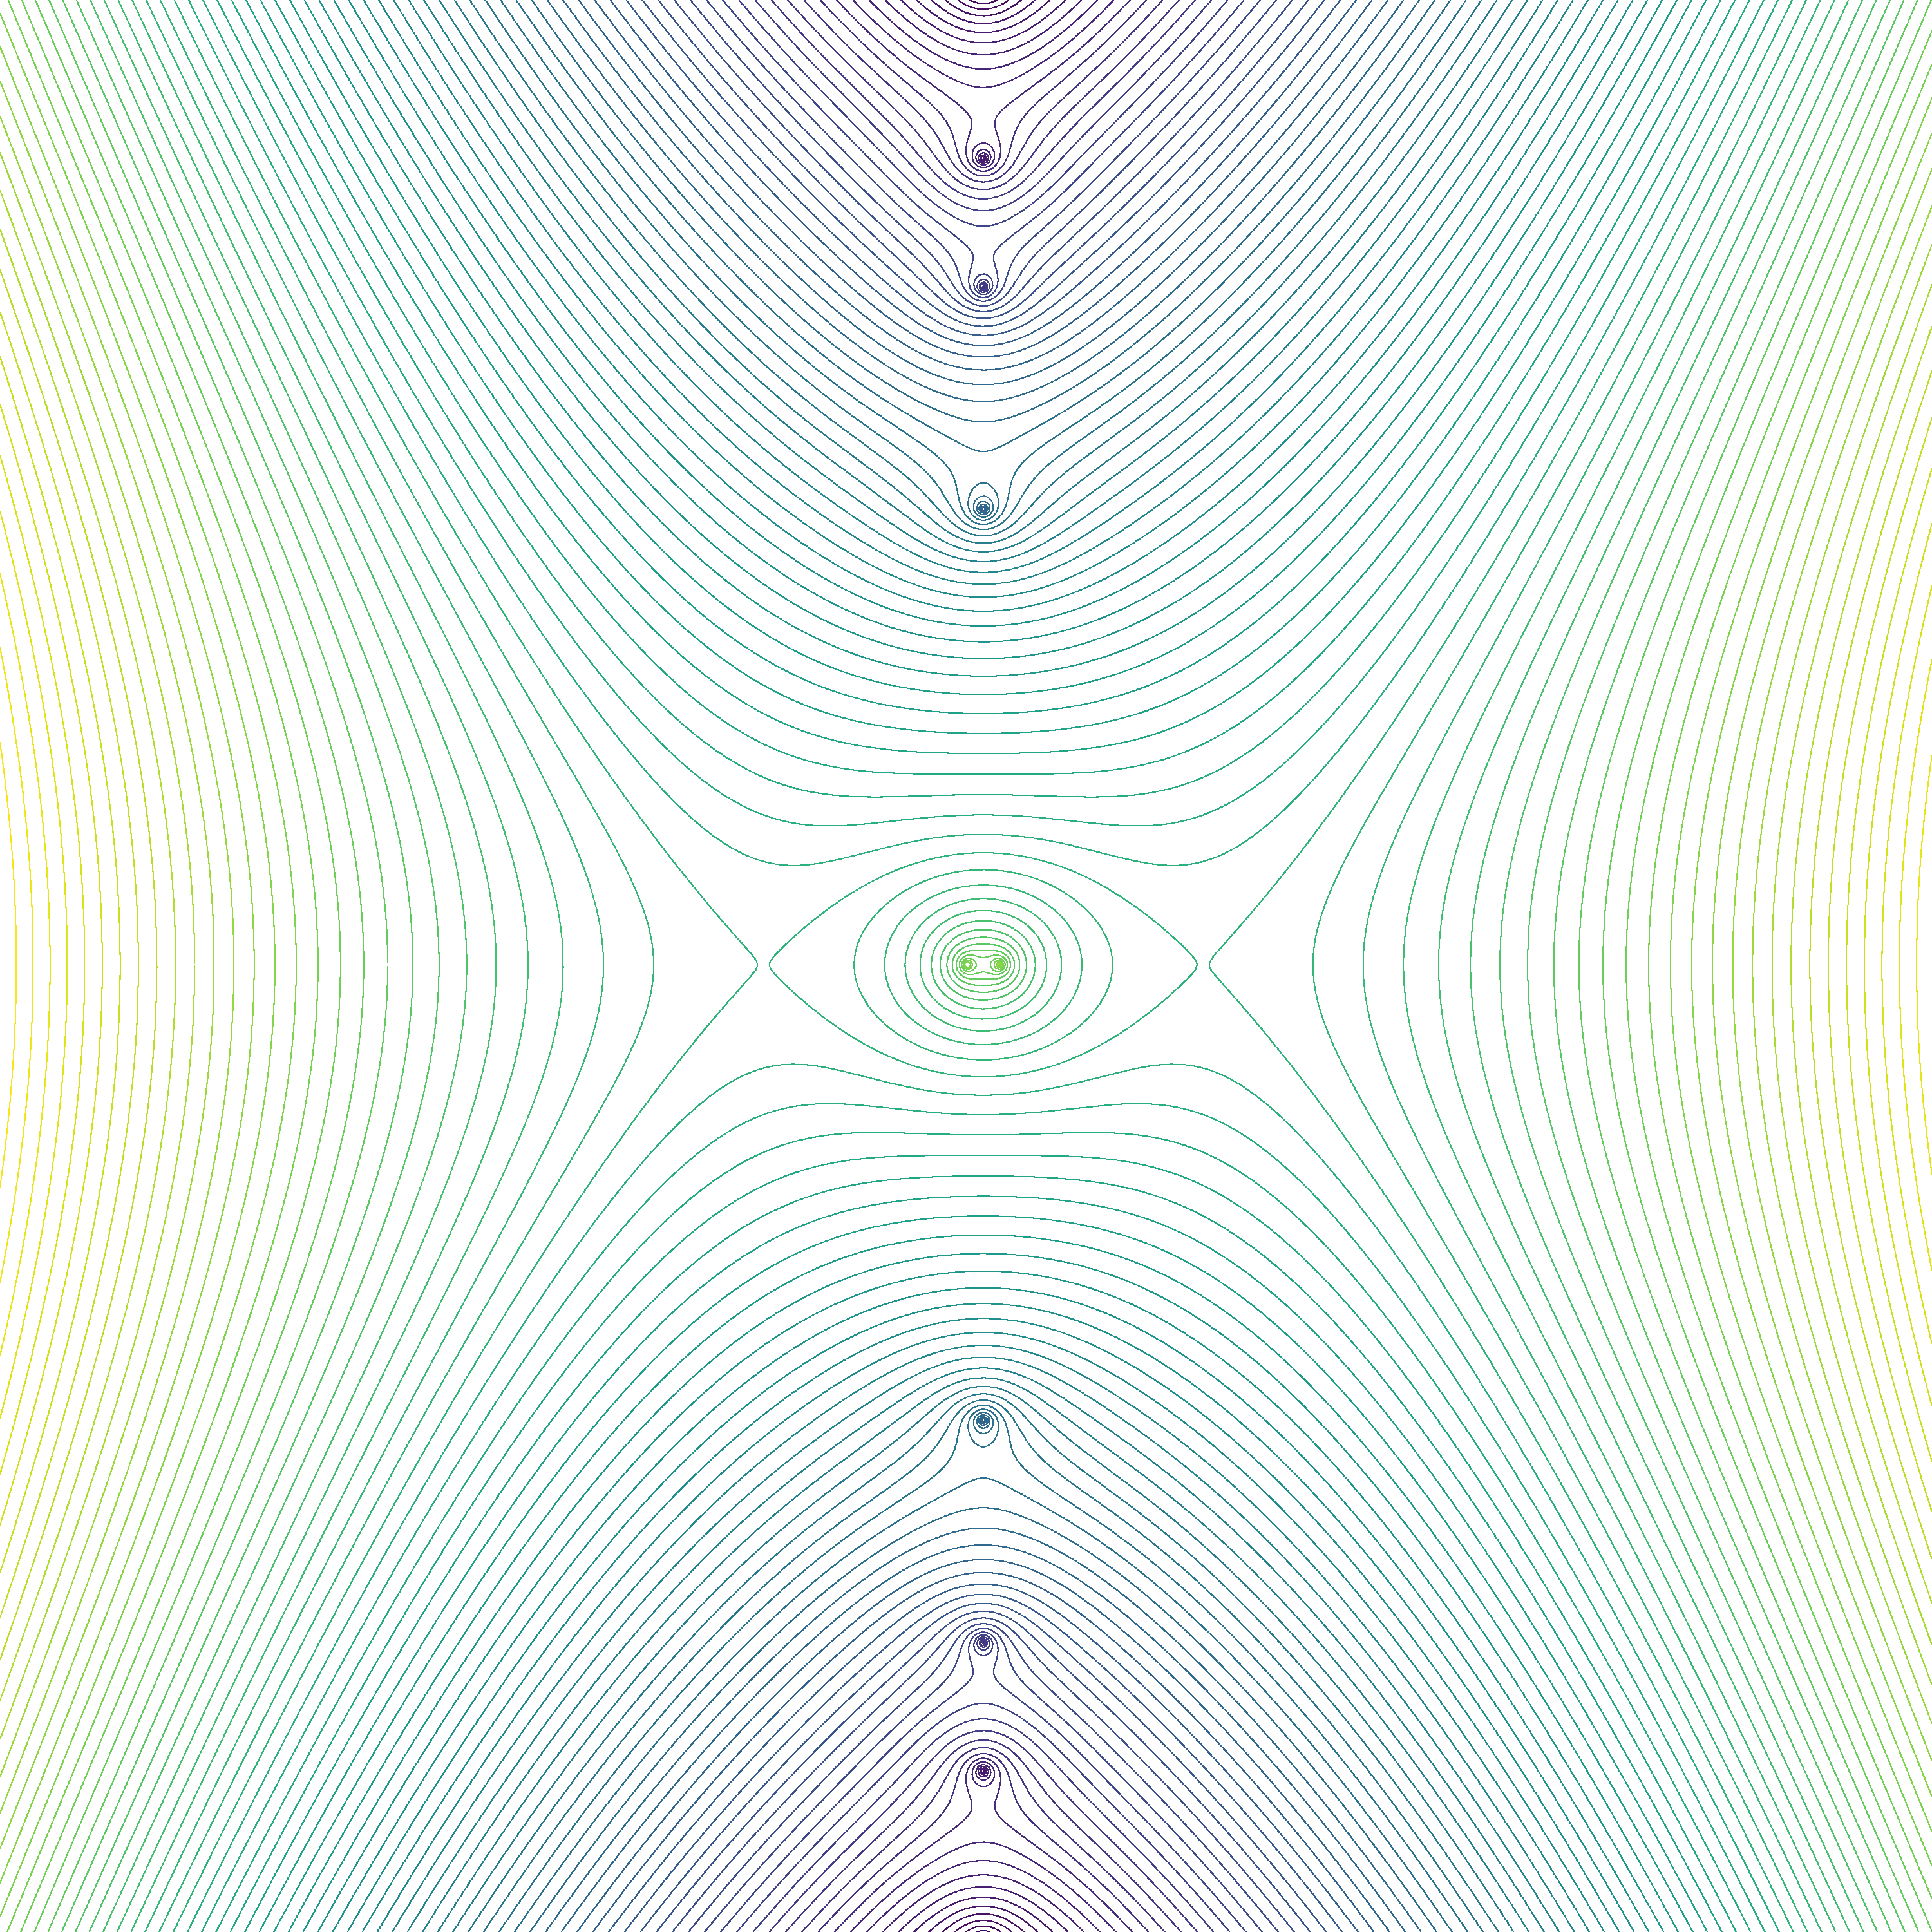
\includegraphics[width=0.55\textwidth]{figures/3030abs_contour_xi.pdf}};
        \begin{scope}[x={(image.south east)},y={(image.north west)}]
            %\draw[help lines,xstep=.1,ystep=.1] (0,0) grid (1,1);
            \foreach \y in {-20,-10,...,20} {
                \node [anchor=east] at (0,\y/60+0.5) {$\y$}; 
                \draw (0,\y/60+0.5) -- (-1mm,\y/60+0.5);
                }
            \foreach \x in {-20,-10,0,1,10,20} { 
                \node [anchor=north] at (\x/56+0.5,0) {$\x$}; 
                \draw (\x/60+0.5,0) -- (\x/60+0.5,-1mm);
                }
            \node[rotate=90] (ylabel) at (-.12,0.5) {$\operatorname{\Im s}$};
            \node (xlabel) at (0.5,-.115) {$\operatorname{\Re s}$};
            \draw[very thin] (0,0) rectangle (1,1);
            \only<2>{\fill[color=white, opacity=0.8] (0.52,0) rectangle (1,1);
            \fill[color=white, opacity=0.8] (0,0) rectangle (0.5,1);}
        \end{scope}
    \end{tikzpicture}%
    \vspace*{-13pt}
    \caption{Betrag der $\xi$-Funktion}
    \end{figure}
\end{frame}
\begin{frame}[label=current]
    \frametitle{Nullstellenverteilung der $\zeta$-Funktion}
    \[
        \zeta(s) = \frac{\pi^{s/2}}{\Gamma(s/2)}\xi(s)  
    \]
    \begin{itemize}
        \item<2-> $\xi(s) = 0$ nur für $0 \leq \Re s \leq 1$.
        \item<3-> Genau für die Polstellen von $\Gamma(s/2)$ gilt $\frac{\pi^{2/s}}{\Gamma(s/2)} = 0$.
        \item<4-> $\implies \frac{\pi^{2/s}}{\Gamma(s/2)} = 0\qquad \forall s \in \{-2, -4, \dots\}$.
    \end{itemize}
    \visible<5->{
        \begin{block}{Folgerung.}
            $\zeta$ besitzt die \glqq trivialen Nullstellen\grqq\ bei $s = -2n,\; n\in \N$ und die Nullstellen von $\xi$, die allesamt im \glqq kritischen Streifen\grqq\  $0\leq \Re s \leq 1$ liegen.
        \end{block}
    }
\end{frame}